\chapter{Chapter 3 - Methodology}
This chapter introduces the reader to the the methodology of the research, investigative work, the subjects under scrutiny and how these leads to the results of this thesis.

\section{International Potential for Free Indoor Mapping Services Survey}
In order to get relevant information regarding the international market for free \glspl{ims}, and to obtain empirical evidence, a survey was conducted. The survey was done at an international level where respondents were asked to reply to a survey estimated to take between six and eight minutes. The main factor in choosing which \glspl{hei} to contact was the size of the institution, as these might have a larger and inherent need and demand for an \gls{ims}. 


The different institutions were contacted exclusively via email, with email and name of institution bein kept in a spreadsheet to avoid double-contacting people and institutions, while enabling the respective contacts of the survey to be re-contacted. Respondents were also welcome to answer the survey in other ways than Google Forms, but no responsents opted for this. Initially, only the absolute highest ranking official of any given institution was contacted, but consequently the invitation letter was altered slightly, to state that any person with relevant experience may answer the survey. The scope was then widened to include anyone from building- and facilites management, property management, information services management and a larger than initially group of senior officials. Media and communications departments were also contacted, as the invitation letter pleaded recipients to forward the letter to whom it might concern. To follow up non-respondents, each respondent was asked to state their email address and affiliation to avoid being contacted after completing the survey. A new list of non-responders was formed throughout the survey period, and sendouts were performed periodically. Furthermore, they were informed that the survey data was to be handled confidentially, and as such every email address from the survey has purposely been redacted in this thesis. The results can be found as a spreadsheet attachment. The first round of send-outs were conducted in March 2016, and the survey was concluded late June the same year. 

\subsection{Purpose of the Survey}
The primary goal of the survey was to assess and evaluate if customers in the \gls{b2bc}-market would be interested in a free \gls{ims}. The secondary goal of the survey was to assess the potential customer's willingness to pay for additional services, as this is crucial for the freemium model to be profitable. Additionally, respondents were asked whether or not an \gls{ims} was desirable in the first place. Lastly, a question was raised regarding the potential concerns in the event of a procurement, concerning demand, price and security concerns.

\subsection{Response Rate, Difficulties and Risks}
The main concern when formulating and conducting the survey at an international level, is in many cases the response rate. Given the importance of the empirical data from the survey, this was a concern from the beginning. 
\newline
\\
The invitation letter was aptly changed to accommodate for any shortcomings the plan for sending out emails had, to increase the number of respondents. Through an iterative process, the invitation letter was changed so that it was made clear that it was possible to answer the survey in a different way than through Google Forms i.e. via telephone or video conference, but none of the respondents opted for this option. Given the low response rate from the initial sendout, telephone calls where considered as means of getting in contact with the correct personnel, but this proved to be time consuming and to little use. During the time of a telephone call, the author would manage to get around ten more contacts through email leading to the abandonment of this method of reaching out. From initially only contacting between one and three individuals from an institution, this number was greatly increased through looking up email addresses from the websites of the respective institutions. This tactic increased the response rate from 5\% to nearly 20\%.  The length of the survey was engineered to be short, as leaders and other senior personnel often have a busy schedule. Additionally, the questions in the survey required little to no knowledge of any technical aspects regarding an indoor mapping solution. This was done in order to appeal to as broad an audience as possible. In total 198 institutions were contacted with 39 answers submitted. A total of 5517 emails were sent, making the average number of emails sent to each institution around 28. 
\newline
\\
During the first phase of the send-out a script handling sending emails spreadsheet was used. As described above, the spreadsheet contained a column with the numerous email addresses, while another column contained the invitation letter. The last two columns contained information whether the institution had already given an answer or didn't want to be involved with the survey, and the last column contained the name of the institution in order to have a better overview. The scripting language itself resembles JavaScript, and runs remotely on Google's servers~\cite{google2016} offering its user seamless integration across the various applications and services provided by Google. The source code of the script was inspired by online tutorials, and was customised for the purpose of sending emails using the information in the spreadsheet. The source code of the script can be seen in Listing~\ref{lst:email}. It should be noted that this way of sending survey invitations was abandoned at a later stage due to inherent limitations in Google's Gmail platform: A limit of 100 recipients per day was simply not enough when the total emails that was due for sending was over 5000. This resulted in abandonment of the script, in favor of using blind copies when sending the huge volume of emails. \gls{ntnu}'s Microsoft Office365 Mail was used instead, as it imposed fewer limitations in number of emails allowed to send during a 24-hour period.


The survey itself was conceived and presented in Google Forms, an easy and widespread method not only for making surveys, but also handling replies in spreadsheet form. The invitation letter contained a short URL of a link to the survey. Appendix B shows the survey as presented to the respondents, and Figure~\ref{fig:contactsheet} shows how respondents were being tracked.


\begin{figure}
    \centering
    \fbox{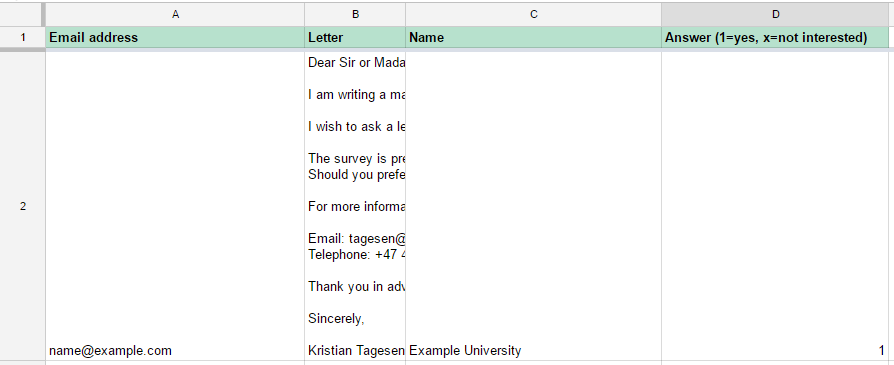
\includegraphics[width=\textwidth]{figs/contactsheet.PNG}}
    \caption{Spreadsheet used to keep track of potential respondents}
    \label{fig:contactsheet}
\end{figure}

\lstdefinelanguage{JavaScript}{
  keywords={break, case, catch, continue, debugger, default, delete, do, else, false, finally, for, function, if, in, instanceof, new, null, return, switch, this, throw, true, try, typeof, var, void, while, with},
  morecomment=[l]{//},
  morecomment=[s]{/*}{*/},
  morestring=[b]',
  morestring=[b]",
  ndkeywords={class, export, boolean, throw, implements, import, this},
  keywordstyle=\color{blue}\bfseries,
  ndkeywordstyle=\color{darkgray}\bfseries,
  identifierstyle=\color{black},
  commentstyle=\color{purple}\ttfamily,
  stringstyle=\color{red}\ttfamily,
  sensitive=true
}

\lstset{
   language=JavaScript,
   extendedchars=true,
   basicstyle=\footnotesize\ttfamily,
   showstringspaces=false,
   showspaces=false,
   numbers=left,
   numberstyle=\footnotesize,
   numbersep=9pt,
   tabsize=2,
   breaklines=true,
   showtabs=false,
   captionpos=b
}

\medskip
\begin{lstlisting}[caption=Email Sendout Script,label={lst:email}]
function sendEmails() {
  var sheet = SpreadsheetApp.getActiveSheet();
  var startRow = 2;  // First mail to send
  var numRows = 73;   // Number of emails to send
  // Fetch the range of cells included in this script
  var dataRange = sheet.getRange(startRow, 1, numRows, 2);
  // Fetch values for each row in the Range.
  var data = dataRange.getValues();
  for (i in data) {
    var row = data[i];
    var emailAddress = row[0];  // First column
    var message = row[1];       // Second column
    var subject = "Market potential for free indoor mapping services - MSc Survey";
    GmailApp.sendEmail(emailAddress, subject, message, {from: 'tagesen@stud.ntnu.no', name: 'Kristian Tagesen'});
  }
}
\end{lstlisting}


\section{Business Model Canvas}
%Skrive hvordan forløpet går gjennom de ulike delene av BMC
This section introduces the reader to the framework that is Business Model Canvas, used to describe the proposed business model in REF(CHAPTER XX). This particular framework has its merits in that it is used to invent, challenge and describe a business model \cite{strategyzer2016}. Further advantages include that it strips away any superfluous elements, improving its readability and enables users and business owners to focus on the most vital elements of a business model. It is also immensely flexible, as changes can be readily made without changing everything thanks to its modular design \cite{osterwalder2013business}. 
\newline
\\
\begin{table}[H]
\centering
\caption{Building blocks of the Business Model Canvas}
\label{tab:canvas}
\begin{tabular}{|l|l|}
\hline
\textbf{Product}                                    & Value proposition     \\ \hline
\multirow{3}{*}{\textbf{Customer interface}}        & Customer segments     \\ \cline{2-2} 
                                                    & Relationship          \\ \cline{2-2} 
                                                    & Distribution channels \\ \hline
\multirow{2}{*}{\textbf{Financial aspects}}         & Cost structure        \\ \cline{2-2} 
                                                    & Revenue stream        \\ \hline
\multirow{3}{*}{\textbf{Infrastructure management}} & Key partnerships      \\ \cline{2-2} 
                                                    & Key activities        \\ \cline{2-2} 
                                                    & Key resources         \\ \hline
\end{tabular}
\end{table}

The framework consists of nine building blocks with varying degrees of importance, but an important relationship between them. When all building blocks are determined, they make up the total strategy of how a business would operate, make money and if desired, capture market shares. Table~\ref{tab:canvas} shows the different building blocks by their respective categories, and Figure~\ref{fig:businessmodelcanvas} shows the empty template for setting up the business model. The business model canvas is described here, as it will serve as a template for the proposal of the business model. Below follows a step-by-step description of the respective building blocks.


\subsection{Customer segments}
This building block consists of the different customer segments a company wishes to concentrate on and reach out to. A market may be single or multi-sided, containing at a minimum a segment per market side. Media companies, credit card companies and to some extent social networking sites among others fall into a multi-sided market category. It is important to note that when offering a value proposition to a market, market size is an important factor, as smaller, niche markets may be a viable market segment as opposed to a bigger market. Finally, diversified products offered through the value proposition may be used to reach smaller subsets of the market.
\subsection{Value proposition}
The value proposition is the building block that describes how a company is different from other competing companies. It details how a company's products or services can create value for their respective customer segments, where values may be qualitative or quantitative. Several means of creating value among customers  includes lower pricing (price-sensitive segments), design (aesthetically appealing products), status (well-known brands), customisation (tailor-made services or products) and performance-driven products. Additionally, introducing a brand new disruptive technology i.e. cell-phones may benefit a business' customer segment, even though it may initially be viewed as unnecessary. Offering consultancy services can also be a value proposition in itself, for instance IT-consultancy services. Concretely, in the framework one wishes to map a value proposition to a particular customer segment, in order to identify the needs of this particular segment.
\subsection{Distribution channels}
Distribution channels concerns how a value proposition is delivered to a customer segment. A channel serves multiple purposes, with the most important being raising awareness around the products or services a company is offering and aiding customers in understanding the value propositions. It also serves a perhaps equally important function in allowing for products or services to be purchased. Furthermore, the channels can be broken into different phases, depending on what phase a product is in. These include:

\begin{itemize}
    \item \textbf{Awareness}: Raising awareness among customers.
    \item \textbf{Evaluation}: How customers are able to evaluate the value proposition.
    \item \textbf{Purchase}: How products are purchasable from the customer's point of view.
    \item \textbf{Delivery}: How a value proposition is delivered to a customer.
    \item \textbf{After sales}: How on-going customer support is handled post-purchase.
\end{itemize}
Along with the next block, Customer relationships, the channels block forms how a business interfaces with their customers. 

\subsection{Customer relationships}
The different types of relationships a business establishes with their respective customer segments are detailed in the customer relationships block. From a business' perspective, having good customer relationships may entail several benefits in increasing their sales volume, gaining new customers and keeping their existing customers from leaving. The perhaps simplest relationship between a business and a customer lies in personal assistance, where actual, dedicated personnel from the business side is serving any customer need from any part of the sales cycle. In a \gls{b2b} market one may have one dedicated person or team per customer, while in a \gls{b2c} market this might not be manageable and call centres or e-mail respondents serves the purpose better. On the flipside, having customers manage themselves entirely either through robust online self-services or inter-customer relationships is also an option depending on the product or service provided. Lastly, co-creation where companies and customers share responsibility for the product is a modern take on a customer relationship, seen in social networks and user-creation oriented services i.e. YouTube.

\subsection{Revenue streams}
How much cash-flow each customer segment generates constitutes the revenue stream building block. It is essential for the profitability of a product or service, with revenue streams being either a one-time fee or recurring payments. Several ways to generate revenue streams include:

\begin{itemize}
    \item \textbf{Subscription fees: }By selling a service, a business may charge its customers of that service for any given time period. 
    \item \textbf{Licensing: }In companies where some form of intellectual property is made, it is possible to generate revenue by the sales or lending of these properties.
    \item \textbf{Advertising: }This type of revenue stream is generated from advertising a product or service on the behalf of some other business entity.
    \item \textbf{Brokerage fees: }By providing services between two parties and taking a fee for the transactions that take place.
    \item \textbf{Asset sale: }Selling the rights to one instance of a product falls into this category, and is the most traditional way of exchanging goods.
\end{itemize}

At this point of setting up the model, the customer segments are linked to its respective value propositions. Each of these should at this point be linked with a revenue stream.

\subsection{Key activities}
The key activities are the detrimental matters that a business needs to attend in order to deliver its value propositions. Together with key resources they are vital in creating and offering the value proposition to the customers, earning revenues and keeping customers satisfied. Consultant and service-oriented businesses often revolve around problem solving as a key activity, helping others with new and existing problems. For manufacturing companies and businesses, proposing, making and delivering products is a key activity, while software and banking service businesses may have a robust platform they offer their customers. In the case of the latter, the platform itself is the main component of their key activities. Lastly, it is important to connect the key activities to the value propositions, as the key activities are the main drivers of the value propositions.

\subsection{Key resources}
The key resources in this framework is absolutely vital for businesses in order to provide and create value propositions for its customers. Together with the key activities, they enable the generation of revenues, maintaining customer relationships and reach markets. Several types of key resources include:  physical (buildings, manufacturing plants), human (consultancy and r\&d services), financial (gaining and edge on competitors by lowering the price point) and intellectual (intellectual properties, brands etc.). The goal 
of the key resources is for the business to surpass competitors on key areas of the key resources.

\subsection{Key partnerships}
This building block concerns the partnerships, suppliers and other third party entities needed to make the business model work. The partnerships can vary in nature, where competitors and non-competitors can forge alliances or creating joint ventures. Any non-in-house solutions have to be supplied by third parties be it manufacturing parts or personnel. Motivations for creating partnerships include optimising the allocation of resources, reducing risk and to cut down on activities not vital in delivering a final product or service. As such, key partnerships can be linked with activities that aren't necessarily key to drive a business' value proposition. 

\subsection{Cost structure}
Different cost structures include fixed costs, variable costs, economies of scope and economies of scale. Fixed costs are volume-independent, and is usually examples of employee salary, rental costs and other facilities. Variable costs are volume-sensitive, while economies of scale concerns the costs changing as a result of a change in the scale of operation. Economies of scope on the other hand benefits businesses that diversify the number of different products or services offered, and is volume-insensitive in this regard. Different cost-structures exist in cost-driven and value-driven models. The former focuses on minimising the costs, and the latter model fits companies that less concerned with price and focuses more on value creation.
Lastly, it is important to note the relationship between cost structures and key activities, as the key activities drive a business' cost structures. 

\begin{figure}[]
\centering
\includegraphics[width=10cm]{figs/busmodcanvas.png}
\caption{Business Model Canvas template. \textcopyright businessmodelgeneration.com}
\label{fig:businessmodelcanvas}
\end{figure}
